\documentclass[a4paper]{article}
\usepackage[utf8]{inputenc}
\usepackage{listings}
\usepackage{parcolumns}
\usepackage{hyperref}
\usepackage{graphicx}
\usepackage{float}
\usepackage{pifont}
\newcommand{\cmark}{\ding{51}}
\newcommand{\xmark}{\ding{55}}
\newcommand{\umark}{\xmark/\cmark}
\newcommand{\dmark}{\cmark/\xmark}
\usepackage{amsmath}
\usepackage{tikz}
\usepackage{makecell}
\usetikzlibrary{shapes.misc, arrows.meta}
\usepackage{array}
\newcolumntype{C}{>$c<$}
\usepackage{color}
\usepackage{fancyhdr}
\usepackage{geometry}
\usepackage[T1]{fontenc}
\usepackage[utf8]{inputenc}
\usepackage{lastpage}
\usepackage{listings}
\usepackage{enumitem}
\usepackage{tabu}
\usepackage[flushleft]{threeparttable}
\usepackage{ulem}
\usepackage{amsmath}
\usepackage{pdfpages}
\usepackage{multicol}
\usepackage{tabu}
\usepackage{parskip}
\usepackage{qtree}
\usepackage{tcolorbox}
\usepackage{scalerel,amssymb}
\def\mcirc{\mathbin{\scalerel*{\circ}{j}}}
\def\msquare{\mathord{\scalerel*{\Box}{gX}}}
\newcommand{\code}[1]{\begin{tcolorbox} \texttt{#1} \end{tcolorbox}}
\def\doubleunderline#1{\underline{\underline{#1}}}
\begin{document}

% COURSE NAME
\title{02110 - Algorithms and Data structrures \\ Fall 2022}

\date{} % blind date
\color{black}
\maketitle
\begin{center}
{ \huge \bfseries Mandatory Assignment 1}\\

\vspace{.25cm}
Daniel F. Hauge \texttt{(s201186)}\\


\vspace{.25cm}
\vfill
\today
\end{center}


\medskip
\newpage

\section{Algorithm proposal}
This assignment propose an algorithm to solve the problem and will utilize dynamic programming techniques and inspiration from the divide and conquer pattern to solve it efficiently.
The optimal solution to the problem can be constructed of solutions to sub problems that could have been computed before, thus memorization can be used.
The optimal solution is found by either picking first or last card plus the optimal solution with rest of the cards where ronald picks first.


The following diagram illustrates a scenario of a given problem at the initial state.
\begin{figure}[H]
    \centering
    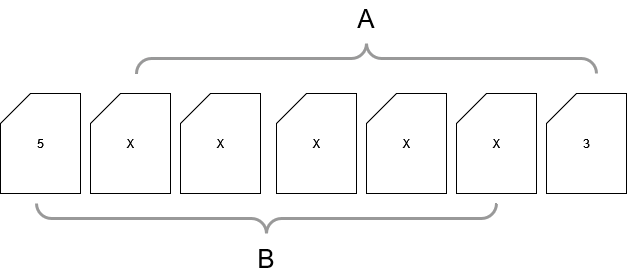
\includegraphics[width=0.6\textwidth]{images/diagram1.png}
    \caption{Diagram illustrating scenario of initial state of a problem}
    \label{fig:D1}
\end{figure}
The optimal solution is then: $\text{Max}\begin{cases}
    5 + \text{Best solution with cards in: }A \\
    3 + \text{Best solution with cards in: }B
\end{cases} $

To continue the example, the following diagram illustrates the scenario where 5 was picked and best solution with cards in A is then needed.
\begin{figure}[H]
    \centering
    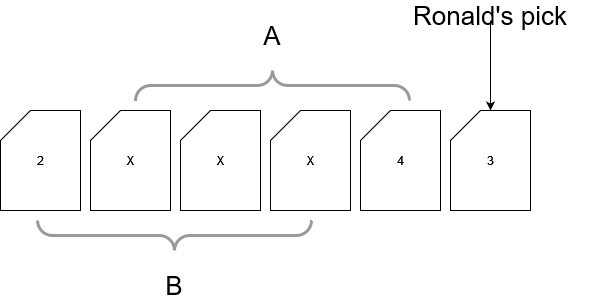
\includegraphics[width=0.6\textwidth]{images/diagram2.png}
    \caption{Diagram illustrating a scenario in which ronald picks next}
    \label{fig:D2}
\end{figure}

With Ronald's strategy being known, one card can be removed and the patterns as in figure \ref*{fig:D1} can be repeated.
This pattern can be repeated in a recursive manner until trivial cases are reached where only 2 or 1 cards remain. 
This algorithm proposal leans towards a top-down dynamic programming approach, as all sub problems and base cases are identified with opportunity for memorization.


\section{Solution}

\begin{itemize}
    \item Given $n$: total amount of cards as integer.
    \item Given $C_i$: as a list of $n$ integers, $C_1, C_2,..., C_n$.
    \item $h$ is defined as head index variable pointing to the leftmost card.
    \item $t$ is defined as tail index variable pointing to the rightmost card.
    \item $M_{i,j}$ is defined as solution to sub problem with the slice of $C$ where $i$ is the leftmost card and $j$ is the rightmost card.
\end{itemize}

Function to find best solution to sub problem where it is Donald's turn to pick a card is defined as follows:

$$ S(h,t) = \begin{cases}
    M_{h,t} & \text{if $M_{h,t}$ found} \\
    0 & \text{if $h = t$} \\
    \text{min}(C_h, C_t) & \text{if $|h-t| = 1$} \\
    \text{max} \begin{cases}
        C_{t-1} + S(h, t-2) \\
        C_h + S(h+1,t-1)
    \end{cases} & \text{if $C_h < C_t$ } \\
    \text{max} \begin{cases}
        C_t + S(h+1, t-1) \\
        C_{h+1} + S(h+2,t)
    \end{cases} & \text{if $C_h > C_t$ } \\
    \text{max} \begin{cases}
        C_{t-1} + S(h, t-2) \\
        C_h + S(h+1,t-1) \\
        C_t + S(h+1, t-1) \\
        C_{h+1} + S(h+2,t)
    \end{cases} & \text{otherwise} \\
\end{cases} $$

The functions captures the reuse of solutions of sub problems that have already been computed to avoid redudant computations, the 2 trivial bases cases, the case where leftmost card is highest, the case where rightmost card is highest and also if rightmost and leftmost are equal.

All succesfull evaluations will be memorized: $M_{h,t} = S(h,t)$, such that the solution is found for any subsequent computation of $S(h,t)$. 

The optimal solution of a given $C$ and $n$ is then found by the following:
$$ Opt_C = \begin{cases}
    \text{max}\begin{cases}
        C_1 + S(2,n) \\
        C_n + S(1,n-1)
    \end{cases} & \text{if $n > 1$} \\
    C_1 & \text{otherwise}
\end{cases} $$

\section{Correctness}
The algorithm ensures correctness by always taking the max of solutions to all sub problems, thus preserving optimal substructures.
With a correct solution to trivial base cases and the ensurance of optimal substructures, a correct complete solution to the original problem can be ensured.

To alleviate potential incorectness from missing details in Ronald's strategy, the algorithm also handles cases where Ronald could pick either leftmost and rightmost because of equality.
\section{Analysis}

\subsection{Time complexity}
% This means the solution can be constructed by a chain of n/2 optimal solutions of sub problems.
In traditional divide and conquer where sub problems are divided by two, thus creating a runtime complexity $O(n\text{ } log\text{ } n)$, this algorithm is a little different.
Considering the context of the function $S(h,t)$ and the disregard of the otherwise and memory cases, then the following reoccurance applies.
$$ T(n) \leq \begin{cases}
    2T(n-2) + c & \text{if } n > 2 \\
    c & otherwise
\end{cases} $$ 

As combining the results, ie. taking max of the two solutions does not take $n$ time, only c is computed for each node considering a recursion tree. 
However, as the recursion is not dividing n by 2, the height is not $log \text{ } n$ but $\frac{n}{2}$.
Therefore we can infer the total amount of leaf nodes to be: $2^{\frac{n}{2}}$. Summing over all levels:

$$ T(n) \leq \sum_{i=0}^{\frac{n}{2}-1} 2^{i}c \leq c (2^{\frac{n}{2}} - 1) $$

With this, the runtime $O(2^{\frac{n}{2}})$ can be speculated, with asymptotic runtime $O(2^{n})$.
If we consider the otherwise case of $S(h,t)$, the runtime will be even worse than what is considered so far. 

The saving grace for the algorithm, is dynamic programming techniques that makes runtime bound by the substructure solution space which is of size $n^2$.
With the runtime bound by solution space, a better runtime complexity that we can infer is: $O(n^2)$ 

Although the worst case runtime complexity is $O(n^2)$ thanks to memoization, in practise it is significantly better.
The following diagram illustrates how the algorithm performs in practise given increasingly larger problems.

\textit{N.B. Card numbers are randomly generated between 1 and 500000}

DIAGRAM OF RUNS


\subsection{Space complexity}

Memory of solutions to subproblems will be stored in $M_{i,j}$.
If every sub problem is evaluated and stored, then the resulting space complexity is O$(n^2)$.
Worst case is very unlikely, and practically it is much less.

In the same manner as time complexity, the following diagram is of space complexity in practise.

DIAGRAM OF RUNS


\end{document}







